\chapter{Batch Size, Dropout and Learning Rate Comparison Data}\label{ch:appAlabel}

%-------------------------------------------------------
%Table of Tests
\begin{table}[H]
\centering
	\caption{Six tests with different Parameter values.}
	\begin{tabular}{| l | c | c | c | c | c | c | c |} 
	\hline
	Parameters & 
	Test1 -\tikzcircle[orange, fill=orange]{3pt}- &
	Test2 -\tikzcircle[blue, fill=blue]{3pt}- &
	Test3 -\tikzcircle[red, fill=red]{3pt}- &
	Test4 -\tikzcircle[lightblue, fill=lightblue]{3pt}- &
	Test5 -\tikzcircle[pink, fill=pink]{3pt}- &
	Test6 -\tikzcircle[turquoise, fill=turquoise]{3pt}- \\ 
	\hline
	Batch Size (train, eval., test) & 
	2 \hfill 2 \hfill 2 & 
	20 \hfill 20 \hfill 20 & 
	20 \hfill 20 \hfill 20 &
	20 \hfill 20 \hfill 20 &
	50 \hfill 20 \hfill 20 &
	50 \hfill 20 \hfill 20 \\
	\hline
	Dropout & 
	0.05 & 0.05 & 0.00 & 0.50 & 0.05 & 0.05 \\
	\hline
	Learning Rate & 
	0.001 & 0.001 & 0.001 & 0.001 & 0.001 & 0.010 \\ 
	\hline
	\end{tabular}
\end{table}
%-------------------------------------------------------

\subsection{Batch Size Test}
%-----------------------------------------------------
%Batch Size Test
\begin{table}[H]
\centering
	\caption{Three tests with different batch size values.}
	\begin{tabular}{| l | c | c | c | c |} 
	\hline
	Parameters & 
	Test1 -\tikzcircle[orange, fill=orange]{3pt}- &
	Test2 -\tikzcircle[blue, fill=blue]{3pt}- &
	Test5 -\tikzcircle[pink, fill=pink]{3pt}- \\
	\hline
	Batch Size & 
	2 \hfill 2 \hfill 2 & 
	20 \hfill 20 \hfill 20 & 
	50 \hfill 20 \hfill 20 \\
	\hline
	Dropout & 
	0.05 & 0.05 & 0.05 \\
	\hline
	Learning Rate & 
	0.001 & 0.001 & 0.001 \\ 
	\hline
	\end{tabular}
\end{table}
	%-------------------------------------------------
	%test error rate
\subsubsection{Accuracy}
\begin{figure}[H]
\centering
	\includegraphics[width=\textwidth]		
	{machine_learning/graph_tests/batch_test/test_error_rate}
	\caption{Test error rate.}
\end{figure}
	%results
\begin{table}[H]
\centering
	\caption{Test error rate results.}
	\begin{tabular}{| l | c | c | c |}
	\hline
	Tests & Value & Epoch & Duration \\
	\hline
	Test1 -\tikzcircle[orange, fill=orange]{3pt}- &
	0.1308 & 25.00 & 0s\\
	\hline
	Test2 -\tikzcircle[blue, fill=blue]{3pt}- &
	0.000 & 25.00 & 0s\\
	\hline
	Test5 -\tikzcircle[pink, fill=pink]{3pt}- &
	0.000 & 25.00 & 0s\\
	\hline
	\end{tabular}
\end{table}
	
%\begin{figure}[H]
%	\centering
%	\includegraphics[width=.5\textwidth]		
%	{machine_learning/graph_tests/batch_test/test_error_rate_values}
%	\caption{Test error rate results.}
%	\label{fig:batch_test_error_val}
%\end{figure}
	%-------------------------------------------------
	%training error rate
\begin{figure}[H]
	\centering
	\includegraphics[width=\textwidth]		
	{machine_learning/graph_tests/batch_test/train_error_rate}
	\caption{Training error rate.}
\end{figure}
	%results
\begin{table}[H]
\centering
	\caption{Training error rate results.}
	\begin{tabular}{| l | c | c | c |}
	\hline
	Tests & Value & Epoch & Duration \\
	\hline
	Test1 -\tikzcircle[orange, fill=orange]{3pt}- &
	0.1148 & 24.00 & 1h 26m 13s\\
	\hline
	Test2 -\tikzcircle[blue, fill=blue]{3pt}- &
	9.5073e-4 & 24.00 & 18m 50s\\
	\hline
	Test5 -\tikzcircle[pink, fill=pink]{3pt}- &
	5.1858e-4 & 24.00 & 14m 50s\\
	\hline
	\end{tabular}
\end{table}

%\begin{figure}[H]
%	\centering
%	\includegraphics[width=.5\textwidth]		
%	{machine_learning/graph_tests/batch_test/train_error_rate_values}
%	\caption{Training error rate results.}
%	\label{fig:batch_test_error_val}
%\end{figure}
	%-------------------------------------------------
	%validation error rate
\begin{figure}[H]
	\centering
	\includegraphics[width=\textwidth]		
	{machine_learning/graph_tests/batch_test/validation_error_rate}
	\caption{Validation error rate.}
\end{figure}
	%results
	
\begin{table}[H]
\centering
	\caption{Validation error rate results.}
	\begin{tabular}{| l | c | c | c |}
	\hline
	Tests & Value & Epoch & Duration \\
	\hline
	Test1 -\tikzcircle[orange, fill=orange]{3pt}- &
	0.1608 & 23.00 & 1h 15m 58s\\
	\hline
	Test2 -\tikzcircle[blue, fill=blue]{3pt}- &
	0.05887 & 23.00 & 17m 21s\\
	\hline
	Test5 -\tikzcircle[pink, fill=pink]{3pt}- &
	0.05418 & 23.00 & 13m 50s\\
	\hline
	\end{tabular}
\end{table}

%\begin{figure}[H]
%	\centering
%	\includegraphics[width=.5\textwidth]		
%	{machine_learning/graph_tests/batch_test/validation_error_rate_values}
%	\caption{Validation error rate results.}
%	\label{fig:batch_test_error_val}
%\end{figure}
	%-------------------------------------------------
	%training avarage loss
\subsubsection{Loss}
\begin{figure}[H]
	\centering
	\includegraphics[width=\textwidth]		
	{machine_learning/graph_tests/batch_test/train_avg_loss}
	\caption{Training average loss.}
\end{figure}
	%results

\begin{table}[H]
\centering
	\caption{Training average loss results.}
	\begin{tabular}{| l | c | c | c |}
	\hline
	Tests & Value & Epoch & Duration \\
	\hline
	Test1 -\tikzcircle[orange, fill=orange]{3pt}- &
	1.639 & 24.00 & 1h 26m 13s\\
	\hline
	Test2 -\tikzcircle[blue, fill=blue]{3pt}- &
	0.06023 & 24.00 & 18m 50s\\
	\hline
	Test5 -\tikzcircle[pink, fill=pink]{3pt}- &
	0.01988 & 24.00 & 14m 50s\\
	\hline
	\end{tabular}
\end{table}	
	
%\begin{figure}[H]
%	\centering
%	\includegraphics[width=.5\textwidth]		
%	{machine_learning/graph_tests/batch_test/train_avg_loss_values}
%	\caption{Training average loss results.}
%	\label{fig:batch_test_error_val}
%\end{figure}
	%-------------------------------------------------
%-----------------------------------------------------

\subsection{Dropout Test}
%-----------------------------------------------------
%Dropout Test
\begin{table}[H]
\centering
	\caption{Three tests with different dropout values.}
	\begin{tabular}{| l | c | c | c | c |} 
	\hline
	Parameters & 
	Test2 -\tikzcircle[blue, fill=blue]{3pt}- &
	Test3 -\tikzcircle[red, fill=red]{3pt}- &
	Test4 -\tikzcircle[lightblue, fill=lightblue]{3pt}- \\
	\hline
	Batch Size & 
	20 \hfill 20 \hfill 20 & 
	20 \hfill 20 \hfill 20 &
	20 \hfill 20 \hfill 20 \\
	\hline
	Dropout & 
	0.05 & 0.00 & 0.50 \\
	\hline
	Learning Rate & 
	0.001 & 0.001 & 0.001 \\ 
	\hline
	\end{tabular}
\end{table}
	%-------------------------------------------------
	%test error rate
\subsubsection{Accuracy}
\begin{figure}[H]
	\centering
	\includegraphics[width=\textwidth]		
	{machine_learning/graph_tests/dropout_test/test_error_rate}
	\caption{Test error rate.}
\end{figure}
	%results
\begin{table}[H]
\centering
	\caption{Test error rate results.}
	\begin{tabular}{| l | c | c | c |}
	\hline
	Tests & Value & Epoch & Duration \\
	\hline
	Test2 -\tikzcircle[blue, fill=blue]{3pt}- &
	0.000 & 25.00 & 0s\\
	\hline
	Test3 -\tikzcircle[red, fill=red]{3pt}- &
	0.030 & 25.00 & 0s\\
	\hline
	Test4 -\tikzcircle[lightblue, fill=lightblue]{3pt}- &
	0.020 & 25.00 & 0s\\
	\hline
	\end{tabular}
\end{table}	
	
%\begin{figure}[H]
%	\centering
%	\includegraphics[width=.5\textwidth]		
%	{machine_learning/graph_tests/dropout_test/test_error_rate_values}
%	\caption{Test error rate results.}
%	\label{fig:batch_test_error_val}
%\end{figure}
	%-------------------------------------------------
	%training error rate
\begin{figure}[H]
	\centering
	\includegraphics[width=\textwidth]		
	{machine_learning/graph_tests/dropout_test/train_error_rate}
	\caption{Training error rate.}
\end{figure}
	%results
\begin{table}[H]
\centering
	\caption{Training error rate results.}
	\begin{tabular}{| l | c | c | c |}
	\hline
	Tests & Value & Epoch & Duration \\
	\hline
	Test2 -\tikzcircle[blue, fill=blue]{3pt}- &
	9.5973e-4 & 24.00 & 18m 50s\\
	\hline
	Test3 -\tikzcircle[red, fill=red]{3pt}- &
	0.000 & 24.00 & 18m 5s\\
	\hline
	Test4 -\tikzcircle[lightblue, fill=lightblue]{3pt}- &
	6.3331e-3 & 24.00 & 18m 10s\\
	\hline
	\end{tabular}
\end{table}		

%\begin{figure}[H]
%	\centering
%	\includegraphics[width=.5\textwidth]		
%	{machine_learning/graph_tests/dropout_test/train_error_rate_values}
%	\caption{Training error rate results.}
%	\label{fig:batch_test_error_val}
%\end{figure}
	%-------------------------------------------------
	%validation error rate
\begin{figure}[H]
	\centering
	\includegraphics[width=\textwidth]		
	{machine_learning/graph_tests/dropout_test/validation_error_rate}
	\caption{Validation error rate.}
\end{figure}
	%results

\begin{table}[H]
\centering
	\caption{Validation error rate results.}
	\begin{tabular}{| l | c | c | c |}
	\hline
	Tests & Value & Epoch & Duration \\
	\hline
	Test2 -\tikzcircle[blue, fill=blue]{3pt}- &
	0.05887 & 23.00 & 17m 21s\\
	\hline
	Test3 -\tikzcircle[red, fill=red]{3pt}- &
	0.05161 & 23.00 & 16m 36s\\
	\hline
	Test4 -\tikzcircle[lightblue, fill=lightblue]{3pt}- &
	0.02366 & 23.00 & 16m 35s\\
	\hline
	\end{tabular}
\end{table}	

%\begin{figure}[H]
%	\centering
%	\includegraphics[width=.5\textwidth]		
%	{machine_learning/graph_tests/dropout_test/validation_error_rate_values}
%	\caption{Validation error rate results.}
%	\label{fig:batch_test_error_val}
%\end{figure}
	%-------------------------------------------------
	%training avarage loss
\subsubsection{Loss}
\begin{figure}[H]
	\centering
	\includegraphics[width=\textwidth]		
	{machine_learning/graph_tests/dropout_test/train_avg_loss}
	\caption{Training average loss.}
\end{figure}
	%results
	
\begin{table}[H]
\centering
	\caption{Training average loss results.}
	\begin{tabular}{| l | c | c | c |}
	\hline
	Tests & Value & Epoch & Duration \\
	\hline
	Test2 -\tikzcircle[blue, fill=blue]{3pt}- &
	0.06023 & 24.00 & 18m 50s\\
	\hline
	Test3 -\tikzcircle[red, fill=red]{3pt}- &
	3.5483e-4 & 24.00 & 18m 5s\\
	\hline
	Test4 -\tikzcircle[lightblue, fill=lightblue]{3pt}- &
	0.09217 & 24.00 & 18m 10s\\
	\hline
	\end{tabular}
\end{table}	
	
%\begin{figure}[H]
%	\centering
%	\includegraphics[width=.5\textwidth]		
%	{machine_learning/graph_tests/dropout_test/train_avg_loss_values}
%	\caption{Training average loss results.}
%	\label{fig:batch_test_error_val}
%\end{figure}
	%-------------------------------------------------
%-----------------------------------------------------

\subsection{Learning Rate Test}
%-----------------------------------------------------
%Learning Rate Test
\begin{table}[H]
\centering
	\caption{Two tests with different learning rate values.}
	\begin{tabular}{| l | c | c | c |} 
	\hline
	Parameters & 
	Test5 -\tikzcircle[pink, fill=pink]{3pt}- &
	Test6 -\tikzcircle[turquoise, fill=turquoise]{3pt}- \\ 
	\hline
	Batch Size & 
	50 \hfill 20 \hfill 20 &
	50 \hfill 20 \hfill 20 \\
	\hline
	Dropout & 0.05 & 0.05 \\
	\hline
	Learning Rate & 0.001 & 0.010 \\ 
	\hline
	\end{tabular}
\end{table}
	%-------------------------------------------------
	%test error rate
\subsubsection{Accuracy}
\begin{figure}[H]
	\centering
	\includegraphics[width=\textwidth]		
	{machine_learning/graph_tests/learning_rate_test/test_error_rate}
	\caption{Test error rate.}
\end{figure}
	%results
\begin{table}[H]
\centering
	\caption{Test error rate results.}
	\begin{tabular}{| l | c | c | c |}
	\hline
	Tests & Value & Epoch & Duration \\
	\hline
	Test5 -\tikzcircle[pink, fill=pink]{3pt}- &
	0.000 & 25.00 & 0s\\
	\hline
	Test6 -\tikzcircle[turquoise, fill=turquoise]{3pt}- &
	0.8992 & 25.00 & 0s\\
	\hline
	\end{tabular}
\end{table}		
	
%\begin{figure}[H]
%	\centering
%	\includegraphics[width=.5\textwidth]		
%	{machine_learning/graph_tests/learning_rate_test/test_error_rate_values}
%	\caption{Test error rate results.}
%	\label{fig:batch_test_error_val}
%\end{figure}
	%-------------------------------------------------
	%training error rate
\begin{figure}[H]
	\centering
	\includegraphics[width=\textwidth]		
	{machine_learning/graph_tests/learning_rate_test/train_error_rate}
	\caption{Training error rate.}
\end{figure}
	%results
\begin{table}[H]
\centering
	\caption{Training error rate results.}
	\begin{tabular}{| l | c | c | c |}
	\hline
	Tests & Value & Epoch & Duration \\
	\hline
	Test5 -\tikzcircle[pink, fill=pink]{3pt}- &
	5.1858e-4 & 24.00 & 14m 50s\\
	\hline
	Test6 -\tikzcircle[turquoise, fill=turquoise]{3pt}- &
	0.9188 & 24.00 & 12m 29s\\
	\hline
	\end{tabular}
\end{table}		
	
%\begin{figure}[H]
%	\centering
%	\includegraphics[width=.5\textwidth]		
%	{machine_learning/graph_tests/learning_rate_test/train_error_rate_values}
%	\caption{Training error rate results.}
%	\label{fig:batch_test_error_val}
%\end{figure}
	%-------------------------------------------------
	%validation error rate
\begin{figure}[H]
	\centering
	\includegraphics[width=\textwidth]		
	{machine_learning/graph_tests/learning_rate_test/validation_error_rate}
	\caption{Validation error rate.}
\end{figure}
	%results
	
\begin{table}[H]
\centering
	\caption{Validation error rate results.}
	\begin{tabular}{| l | c | c | c |}
	\hline
	Tests & Value & Epoch & Duration \\
	\hline
	Test5 -\tikzcircle[pink, fill=pink]{3pt}- &
	0.02661 & 23.00 & 13m 50s\\
	\hline
	Test6 -\tikzcircle[turquoise, fill=turquoise]{3pt}- &
	1.152 & 23.00 & 11m 29s\\
	\hline
	\end{tabular}
\end{table}		
	
	%-------------------------------------------------
	%training avarage loss
\subsubsection{Loss}
\begin{figure}[H]
	\centering
	\includegraphics[width=\textwidth]		
	{machine_learning/graph_tests/learning_rate_test/train_avg_loss}
	\caption{Training average loss.}
\end{figure}
	%results

\begin{table}[H]
\centering
	\caption{Training average loss results.}
	\begin{tabular}{| l | c | c | c |}
	\hline
	Tests & Value & Epoch & Duration \\
	\hline
	Test5 -\tikzcircle[pink, fill=pink]{3pt}- &
	0.01988 & 24.00 & 14m 50s\\
	\hline
	Test6 -\tikzcircle[turquoise, fill=turquoise]{3pt}- &
	12.56 & 24.00 & 12m 29s\\
	\hline
	\end{tabular}
\end{table}		
	
	%-------------------------------------------------
%-----------------------------------------------------
